\documentclass[a4paper]{article}

\usepackage[utf8]{inputenc}
\usepackage[francais]{babel}

\usepackage{graphicx}
\usepackage{fullpage}
\usepackage{amsfonts}
\usepackage{amsmath}

%\setlength\parindent{0pt}

\title{Projet - ASR1} 
\author{Rémy Grünblatt\\Simon Mauras}
\date{5 janvier 2015}

\begin{document}
  
  \maketitle

  \section*{Introduction}

  L'objectif de ce projet est de réaliser à l'aide du logiciel logisim un processeur 16 bits avec pipeline. La première partie a pour objectif d'obtenir une première version fonctionnelle. La seconde ajoute une logique Bypass. La troisième partie introduit des entrées/sorties à l'aide du Mapping Memory. Enfin la quatrième partie consiste en l'ajout des logiques Stall et Stomp pour résoudre les derniers problèmes liés au sauts.

  Ce projet à été réalisé par Rémy Grünblatt et Simon Mauras, élèves en L3 au département d'info de l'ENS de Lyon. Les fichiers logisim, les codes assembleurs de test et les sources du compilateur sont disponibles dans l'archive fournie.

  \tableofcontents
  
  \newpage
  
  \section{Un processeur avec pipeline}
  
  \subsection{Correction du programme assembleur}
  Le programme assembleur suivant est incorrect car l'instruction \verb|lui| doit être utilisée avec un immédiat de 10 bits au plus (celui ci étant décalé de 6 bits vers la gauche afin d'obtenir un entier 16 bits).
\begin{verbatim}
lui r2, 0x8000
lw r1, r2, 1
\end{verbatim}
  Une version correcte serait donc: 
\begin{verbatim}
lui r2, 0x200
lw r1, r2, 1
\end{verbatim}
  Cependant, pour le moment notre pipeline ne peut utiliser la valeur d'un registre qu'après un laps de deux cycles. Nous ajoutons donc :
\begin{verbatim}
lui r2, 0x200
nop
nop
lw r1, r2, 1
\end{verbatim} 

\subsection{Tests}
Voici deux programmes nous ont permis de tester le bon fonctionnement de notre pipeline :
\begin{verbatim}
# --------------------------------------------------
# Programme qui compte jusqu'a 10

# À chaque modifiaction d'un registre, deux cycle sont exécutés avant
# que la nouvelle valeur soit utilisable...

# À chaque BEQ ou JALR, deux instructions sont exécutées par le pipeline
# avant modification du registre PC...

         addi r2, r0, 10
         addi r1, r0, 0
         nop                     # Deux cycles sont nécessaires avant
         nop                     # de pouvoir utiliser r1
loop:    beq r1, r2, endloop
         nop                     # Deux cycles s'écoulent avant la
         nop                     # modification du PC
         addi r1, r1, 1
         beq r0, r0, loop
         nop                     # Deux cycles s'écoulent avant la
         nop                     # modification du PC
endloop: halt

# --------------------------------------------------
# Programme qui calcule la différence de deux entiers

addi r1, r0, 30
addi r2, r0, 16
nop
nop
nand r3, r2, r2  # Complément à 1 de 16
nop
nop
addi r3, r3, 1   # Complément à 2 de 16
nop
nop
add r4, r1, r3   # Soustraction
nop
nop
halt
\end{verbatim}

  \section{Un pipeline avec logique bypass}
  
  \subsection{Remarques}
  
  Nous avons pris dans cette partie deux initiatives. Si deux instructions consécutives modifient un registre et qu'une troisième la lit à la suite, la valeur la plus récente doit être utilisée. De plus, lorsqu'une instruction écrit une valeur dans le registre \verb|r0|, la logique bypass ne doit pas renvoyer celle-ci.

  \subsection{Correction du programme assembleur}
  
  Avec la logique bypass, nous avons corrigé le bug lié au fait que la valeur de \verb|r2| ne peut être utilisée que deux instructions après \verb|lui|. Cependant ce laps de deux cycles est aussi présent pour les sauts. Les deux instructions qui suivent un \verb|beq| ou un \verb|jalr| sont donc systématiquement exécutées. Un problème peut se poser avec le programme suivant :
\begin{verbatim}
lui r2, 10
beq r1, r2, label
addi r2, r2, 1
\end{verbatim}
  Il nous faut donc le modifier ainsi :
\begin{verbatim}
lui r2, 10
beq r1, r2, label
nop
nop
addi r2, r2, 1
\end{verbatim}

  \subsection{Tests}
  Nous avons repris le programme nous permettant de faire la soustraction de deux entiers, en enlevant les instructions \verb|nop| devenues inutiles avec la logique bypass.

  \section{Mapping Memory}
  
  \subsection{Choix de segmentation}
  
  Nous avons choisis d'implémenter Keyboard, TTY et Video Card.
  \begin{itemize}
  \item L'adresse \verb|0xFFE0| est réservée pour le clavier (en lecture)
  \item L'adresse \verb|0xFFEF| est réservée pour la sortie TTY (en écriture)
  \item Les adresses \verb|0xFFF0| à \verb|0xFFFF| sont réservées pour l'écran (en écriture).\\ Celui-ci est de taille 16x16, chaque entier correspond à une ligne (16 bits).
  \end{itemize}
  
  \subsection{Tests}
  
  \begin{center}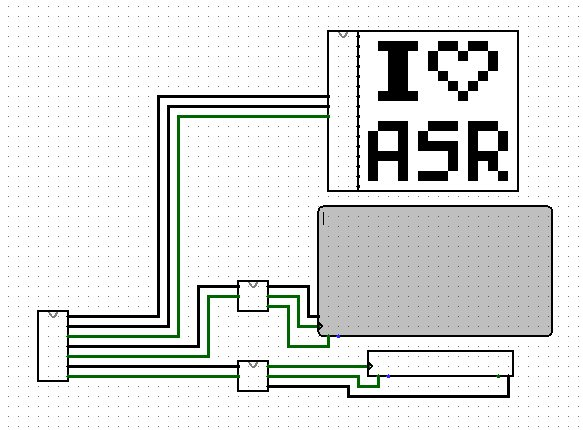
\includegraphics[width=10cm]{screen.jpg} \\ Rendu obtenu lors de l'écriture sur l'écran\end{center}

  Nous avons testé les périphériques TTY et keyboard avec le programme suivant :
\begin{verbatim}
# ------------------------------------------------------------------------------------
# Un programme qui écrit en majuscule (sur TTY) ce que l'utilisateur rentre (keyboard)

        movi r1, 0xFFEF   # TTY
        movi r2, 0xFFE0   # KEYBOARD
        movi r3, 0x8000   # Negative integer ?
        movi r6, 0x7FFF
        movi r7, 0xFFFF
begin:  lw r4, r2, 0      # read
        movi r5, -97
        add r5, r4, r5
        nand r5, r3, r5
cond1:  beq r5, r6, endif # Si le caractere est avant 'a' (r4 - 97 < 0)
        nop
        nop
        movi r5, -123
        add r5, r4, r5
        nand r5, r3, r5
cond2:  beq r5, r7, endif # Si le caractere est après 'z' (r4 - 126 >= 0)
        nop
        nop
        addi r4, r4, -32  # miniscule -> MAJUSCULE
endif:  sw r4, r1, 0      # write
        beq r0, r0, begin
        nop
        nop
        halt
\end{verbatim}

  \section{Un pipeline avec logique Stall et Stomp}
  
  Pour tester la logique Stall et Stomp, nous avons simplement réutilisé le programme permettant de passer une chaine de caractère en majuscule en retirant les instruction \verb|nop| devenues inutiles.

  \section{Compilateur}

  À la fin de ces quatres parties nous avions l'envie d'implémenter un programme plus conséquent. Nous avons choisis de faire un petit compilateur partant d'un langage purement impératif avec des pointeurs basiques vers du code assembleur RISC-16. Il est ainsi plus simple de programmer rapidement et sans bug des programmes plus long.

Le compilateur est écrit en OCaml et utilise OCamllex et OCamlyacc. Il commence l'analyse d'un programme en attribuant un identifiant à chaque variable qui apparaît. Les valeurs sont stockées dans la RAM, sont lues au début d'une instruction et sont enregistrées en fin d'instruction. Aucune optimisation n'a été faite pour l'utilisation des registres.

Pour éviter de devoir enregistrer plus de 8 résultats intermédiaires, il n'est pas possible de faire de calcul avec plus de deux opérandes.

Un des problèmes que nous avons rencontré est l'impossibilité de faire des sauts plus grands que 64 instructions dans le code source. En effet le corps d'une boucle \verb|while| peut tout de suite devenir très conséquent. Nous avons commencé par manuellement décomposer un long saut en plusieurs petits. Cependant le code devenait très vite pollué car un grand nombre de ligne doit parfois être ajouté. Nous avons donc décidé d'utiliser l'instruction \verb|jalr| pour l'implémentation des structures \verb|while| et \verb|if then else|.

  \begin{center}
    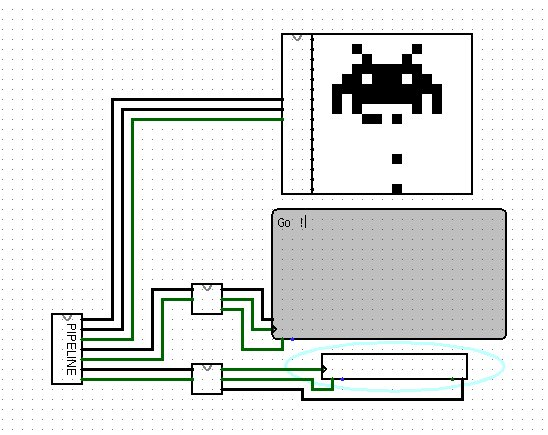
\includegraphics[width=10cm]{space_invaders.jpg}\\
    Rendu d'un programme compilé avec le compilateur
  \end{center}

\end{document}
